% vim:textwidth=70
\chapter{自动推断系统层次结构任务模型的方法}
\label{chap:scalpel}

\section{本章引言}

随着Internet服务逐渐进入人们日常的生产生活,它们的可靠性也变的越来
越重要。系统设计实现上的缺陷,一直伴随着这些服务而生,导致服务性能下降,
甚至彻底中断运行。在诸多的软件缺陷(bug)中,那些最难找到和解决的是让
系统仍然运行,但是却偏离了系统期望行为的缺陷。这些缺陷的根本原因,隐藏
在复杂甚至是混乱的应用逻辑中,因此寻找并分析这些缺陷变的异常困难。

支撑Internet服务的系统本质上就非常复杂,这更增加了分析理解系统异常行为
的难度。这些系统通常使用了分层的体系结构,将其功能抽象表达为不同的层次
结构。其运行时具有高度的并发性。系统在运行时,处理着许多用户层次的
\emph{任务},例如用户请求,任务被分成许多阶段执行,不同的阶段被分布在
多个机器、进程和线程上执行,使用事件或者异步消息作为通知机制。验证单独
每个任务的行为,是一件具有挑战性的问题,因为开发人员需要重构出任务的执
行流,将任务执行过程中的各个阶段重新连接起来。

% xxx:PacificA

从概念上说,开发人员可以把任务执行表示为\emph{层次结构的任务模型},这
与系统的分层体系结构设计一致。任务模型中的任务表示在系统不同函数抽象层
次的执行过程。高层任务的执行被分为若干低层子任务。以PacificA为例,
PacificA是一个类似BigTable的分布式存储系统。图~\ref{xxx}显示了用户向
PacificA提交数据的任务执行层次。数据提交任务被分为两步(图的右边),分
别处理本地数据提交和远程数据提交。每个任务分别由若干{叶子任务}构成,叶
子任务的边界由{同步点}确定。。基于任务模型,开发人员可以更好的理解系统
层次模块间的结构,以及不同模块间的依赖关系,并验证处于不同层次任务的行
为。

然而,目前的工具需要开发人员手动标注任务模型。例如,Pip~\cite{pip}要求
开发人员将系统预期行为,用“期望(expectations)”的形式表达,“期望”
表达了系统正确执行时的任务模型,包括对执行时资源使用的约束。通过对比期
望与实际执行的区别,可以验证系统运行时行为。写出一个全面表达系统高层设
计与底层实现的期望是非常困难的并容易出错的事情,特别对那些正在快速发展
中的系统。基于执行路径的工具,例如Magpie~\cite{magpie},可以从运行时事
件trace推断每个请求的执行路径,但是它仅可以处理的一组事前确定的事件,
并且需要开发人员指定任务的边界与关联条件。

本文的目的是探索不需要人工帮助,自动推断层次结构任务模型的方法。开发人
员不需要手动标注源代码来指定任务边界,并且任务的层次结构也应该能够自动
推断得到。这是完成自动分析诊断复杂系统目标的必要条件。开发人员和系统管
理员可以利用得到的任务模型,以可视化的形式表现系统设计和实现,也可以将
任务模型作为输入,使用其它工具调试或验证系统设计。

设计一个自动推断任务模型的工具面临如下几个挑战性问题。首先,应该能够确
认合理的任务边界,这一过程应该只基于对系统执行过程的监视,而不需要开发
人员显式的标注。其次,必须能够正确的关联任务之间依赖关系。特别是,必须
能够辨别任务之间因为共享资源(例如,共享队列、锁等)而产生的依赖关系。
最后,应该能够自动恢复任务的层次结构。任务由许多或者顺序或者并行的子任
务构成。考虑到复杂系统中任务执行的非确定性,确定它们的依赖关系与层次结
构并不容易。

在本文中,我们描述了如何自动推断复杂系统层次结构任务模型的方法,并实现
了一个推断工具Scalpel。我们通过使用插装(instrument)技术来透明的观测
系统运行,获取系统运行过程的trace,包括应用层函数和系统同步函数的调用
(例如signal/wait)。推断过程使用trace作为输入,自下而上(bottom-up)
的推断系统层次结构任务模型,推断的过程分为三步,分别对应上面提到的三个
挑战性问题。

首先,我们将运行过程分为一个个叶子任务,它们是层次结构任务模型中最基本
的任务。叶子任务的边界对应执行过程的同步点(synchronization point)。
在同步点,线程或进程相互同步从而具有因果依赖关系,因此同步点是推断任务
边界的一个合理启发(heuristic)。

其次,我们按照运行时的因果依赖关系,将叶子任务用有向边连接,形成一个因
果关系图。叶子任务的因果依赖关系由任务运行时的
happened-before~\cite{lamport_clock}关系推断得到。

最后,我们在任务关系图上,推断出层次结构。每一个层次,大致对应系统设计
与实现上的一个层次。我们使用聚类算法寻找任务因果关系图上重复出现的模式
(频繁子图),以此为依据确认高层任务与构成它的子任务。通过递归的使用聚
类算法,我们能够进一步寻找更高层次的任务。

我们分别在Apache Web服务器和PacificA上应用Scalpel,结果显示,Scalpel的
推断方法能够得到具有合理意义的任务模型,并且完全不需要开发者的手工标注。
进一步,Scalpel能够帮助开发者解决PacificA中的一个性能问题,该问题导致
PacificA对网络带宽的利用率只有最大值的70\%。

\note{文章安排}

\section{推断方法设计}

本节叙述推断方法设计,以及它的原型实现\pozhehao{}Scalpel。

\subsection{收集系统运行trace}

我们使用插装技术透明的观测系统运行,收集运行过程的函数调用,以及调用参
数,包括应用层函数和系统同步函数(signal/wait)与系统Socket调用
(send/recv)。默认所有的函数调用都会被收集到trace。

% xxx: 全序?

\subsection{确定叶子任务}

在系统运行trace的基础上,我们首先需要确定叶子任务的边界。Scalpel使用
\emph{同步点}作为启发定义任务边界。同步点是两个线程同步相互执行,从而
具有happened-before关系的地方。在同步点,线程可能因为互斥或者相互协同
而具有happened-before关系,前者的例子是线程等待另一个线程释放保护共享
资源的锁,后者的例子是线程向另一个等待在event上线程发signal消息,通知
对方继续执行。

我们定义两个相继的同步点之间的执行为一个叶子任务。采用这个定义的原因是,
首先两个同步点之间的一段执行是相对独立,并且自包含的,不与其它线程的执
行相互依赖。因此,它们合理的成为任务模型中最小粒度的一段执行,也是叶子
任务的一个自然定义。另外,因为采用了同步点定义叶子任务的边界,叶子任务
之间的依赖关系也只发生在边界之间。

Scalpel通过插装系统函数库中的同步原语(锁、信号、事件等)与socket操作
\footnote{我们认为通信也是一种同步操作。}记录同步点操作。在实际系统中
的应用经验表明,插装这些系统操作是足够的。如果应用系统使用spin-lock或
者lock-free的数据结构,则仅插装系统调用是不够的。这时Scalpel会丢失一些
同步点从而使任务模型粒度更粗。手工标注可以解决这个问题,但是整个推断方
法不再是全自动的。鉴于多数实际系统还是采用系统调用进行同步,我们将这个
问题留作将来的工作。

\subsection{任务因果关系图}

% xxx: recall the happened-before relation somewhere?

为了推断任务的层次结构,我们首先要连接叶子任务之间的因果关系。我们使用
有向图表示任务之间的关系。这个图中,节点表示叶子任务,有向边表示叶子任
务之间的的因果依赖关系。例如在PacificA中(图~\ref{xxx}),当存储的主节
点收到用户提交数据的消息后,首先将数据在本地持久化存储
(\texttt{Logic\-Replica\-::Mutate}),之后将数据用异步RPC的方式发送给
次节点(\texttt{Rpc\-Client\-::RpcAsync\-Call\-Chain})。因此这两个叶
子任务之间用有向边连接。

Scalpel使用happened-before关系推断任务的因果依赖关系,这包括同一线程内
顺序执行的两个叶子任务,以及因为同步而依次执行的叶子任务。并不是所有因
为同步而具有happened-before关系的叶子任务都存在因果关系。一个“真”的
依赖关系的例子是,一个从队列里取出并处理事件的任务,在因果关系上依赖于
产生那个事件并将其加入队列的任务。另一方面,如果两个线程使用互斥锁同步
对共享资源(例如I/O)的访问,虽然它们的行为构成happened-before关系,但
实际上,任务之间并不相互依赖,其执行的顺序由调度器随机决定。

Scalpel使用若干启发区分这两种不同的关系。如果系统使用操作系统提供的队
列(例如I/O completion ports,IOCP),或者通知机制(例如event),则可
以使用同步操作使用的句柄(保存在插装得到的trace中,是同步操作的参数),
将生产线程与消费线程联系起来。对于操作系统的互斥(mutex)与信号量
(semaphore)对象,它们通常仅仅被用来同步线程对共享资源的访问,生产线
程和消费线程之间通常会使用显式的通知机制(IOCP等)协调数据共享,因此不
认为它们构成因果依赖关系。

对于使用TCP通信的因果关系,由于TCP的数据流语意会让消息的边界无法分辨,
因而目前只能依赖程序员提供额外信息(例如在消息中做标记)连接消息的发送
者和接受者,否则Scalpel无法准确匹配。然而这会引入手工干预。

% xxx:TCP边界,怎么说。

\subsection{推断任务层次结构}

我们通过不断挖掘任务因果关系图上重复出现的模式,来推断任务的层次结构。
发掘算法受到文章~\cite{wpp}的启发,\cite{wpp}的工作通过搜寻“热点子路
径”(就是函数调用路径上重复出现的字串),来推断上下文无关文法。类似的,
我们的算法搜寻任务因果关系图上重复出现的子图。我们认为每一个子图都在逻
辑上代表了一个更高层的任务,它由子图中的任务集合构成。通过递归调用挖掘
算法,我们得到了层次结构的任务模型。

具体的,推断算法首先枚举任务因果关系图上所有的连通子图,并将这些子图按
照相似度(在下文中叙述)聚类为多个模式。推断算法将每个出现次数超过设定
阈值的模式定义为一个高层任务。接下来,得到的高层任务被替换为单个“超级”
节点。通过递归应用算法,我们可以得到更高层的任务,直到没有新的高层任务
产生。这时,因果关系图包括了若干超级节点,以及一些未聚类的叶子节点,图
可能是连通也可能是不连通的。Scalpel将那些超级节点输出,每个节点都是一
个最高层的任务模型。通过将超级节点展开为构成它们的子图,我们可以得到任
务的整个层次结构。

算法中使用相似度将子图聚类为不同的模式,目前,我们使用精确匹配来定义两
个子图相似,也就是两个子图完全同构。我们使用确定性的序列化算法,将子图
编码,并使用编码的哈希值将子图聚类。这个聚类算法非常有效。当编码叶子任
务时,我们使用任务两个边界上的函数调用栈作为任务的编码,忽略了任务执行
过程中调用的函数。对
% xxx \footnote{\note{有二义性,没弄明白,看看代码。}}
于同一个类中的叶子任务,它们的函数调用栈完全相同。这个方法忽略了叶子任
务一些不重要的区别,例如函数的参数与线程号。从经验来看,这个方法很好的
区分了同一类别的叶子任务。

% xxx \note{具体算法(伪代码)}


\subsection{实现}

% xxx
a

\section{讨论}

Scalpel主要是为系统开发者而设计的,希望能够帮助他们理解、验证与调试搭
建的系统。因此,我们假设程序的调试信息(主要是符号表)是可以得到的。
Scalpel利用这些信息追踪函数调用,为叶子任务提供易于理解的名字。这个假
设并不是推断任务层次结构的必要条件。即使没有调试信息,我们仍然可以对系
统调用插装,追踪同步点的调用信息。通过使用stack walking技术,我们可以
得到函数地址形式的调用栈。函数地址与函数名有对应关系,仍然可以用来分析
推断任务结构。因此,无论有没有调试信息,我们都可以推断出同样结构的层次
任务模型来。如果没有调试信息,叶子任务的名字不易于人去理解,但是不妨碍
使用其他调试工具分析任务模型。

人们习惯上使用因果路径分析~\cite{pinpoint, project5, pip, magpie}去分
析系统行为,这种方法将系统的运行过程抽象为单层的因果路径。我们认为,作
为本文核心概念的层次结构任务模型,是对因果路径分析的一个扩展。实际上,
如果只看叶子任务这一层,则我们的任务模型实际上就是因果路径,因此也可以
被用在类似的基于路径的分析中。然而,层次结构可以带来更多的好处。它将实
现细节包装在更高层次的任务中,程序员可以再不同的任务层次和粒度下,分析
验证系统行为。可以用类似Pip~\cite{pip}的方法,在不同层次的任务上,将
系统行为与程序员的期望做比较验证。虽然本文的工作侧重与推断方法的设计,
并未提出在任务模型上进一步分析的方法,我们希望能在将来的工作中完成进一
步的工作。

\section{验证推断方法}

iocp, event, mutex
% xxx

\section{应用实例}

在本节,我们使用Scalpel分析一些复杂系统,以评测任务模型是否有效。可以
从两个方面来评测任务模型。首先,任务模型应该能够表达出系统设计的含义。
这一点很难用数字测量,因此,我们需要程序员去将推断的任务模型与实际系统
设计对比,判断任务模型是否表达了系统设计的某些方面。其次,任务模型也是
验证系统正确性或者性能的方法,所以,我们也可以评测任务模型在帮助调试系
统时的有效性。

我们同时使用这两种方式评测Scalpel,分别将Scalpel应用在
Apache~\cite{apache}和PacificA~\cite{pacifica}上。Apache和PacificA都使
用了典型的配置。我们在Apache上增加了一个Subversion(SVN)模块,并使用
客户端执行10次checkout。我们使用两台机器配置了一个PacificA的复制组
(Replication Group),一台机器是主节点(primary),一台是从节点
(backup)。我们运行一个测试程序,在Pacifica中创建一个表,并提交15条随
机数据。我们使用Scalpel追踪每个系统的运行,并推断任务模型。两个实验都
是在如下机器配置上进行的:2.0 GHz Xeon双核CPU,4 GB内存,运行Windows
Server 2003 SP2操作系统,机器间通过1 Gb网络连接。

\subsection{Apache}

我们首先人工验证Scalpel在Apache上推断的任务模型。图~
\ref{fig:apache_model}显示了得到的模型。在图上,每个节点都是一个叶子任
务,连接任务的实线与虚线表示任务之间的因果关系,实线表示线程内部执行顺
序因果关系,虚线表示线程间因果关系。叶子任务上标记了任务起始点的调用栈。
为了易于理解,在本文中,我们只显示了调用栈尾部调用同步函数的那个函数名
称。

\begin{figure}
\centering
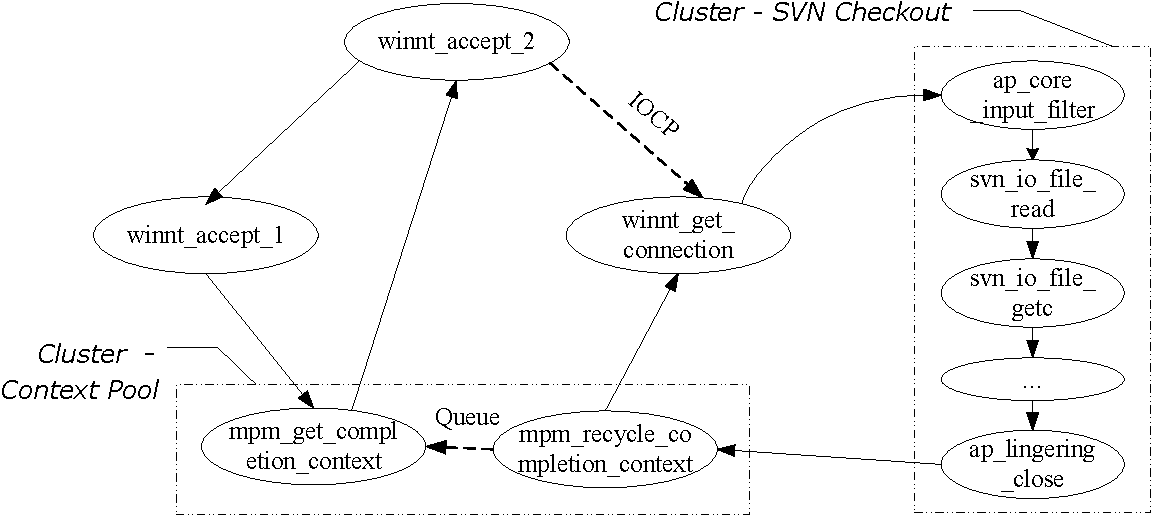
\includegraphics[width=\linewidth]{apache-task-model}
\caption{执行SVN checkout得到的Apache任务模型}
\label{fig:apache_model}
\end{figure}


通过仔细阅读理解Apache和SVN的代码,我们确定推断的模型就是Apache服务SVN
checkout操作时的工作流程。Apache接受外来的请求,并将请求交给线程池中的
一个worker线程去完成。Scalpel推断出5个Apache核心执行的叶子任务(图~
\ref{fig:apache_model}的左边部分)。每个任务表示Apache接受并服务请求的
主要步骤。详细说,监听线程接受连接(\texttt{winnt\_accept\_1}),从连
接上下文\footnote{Connection context,描述外来请求的数据结构。}资源池
中取出一个连接上下文(\texttt{mpm\_get\_completion\_context}),并将这
个上下文通过I/O completion port(IOCP)传递给worker线程
(\texttt{winnt\_accept\_2}),并继续等待其他请求到来。在IOCP的另一边,
线程池中的一个worker线程首先获得连接上下文
(\texttt{winnt\_get\_connection}),并调用SVN服务模块去处理请求(从
\texttt{ap\_core\_input\_filter}到\texttt{ap\_lingering\_close})。之
后,worker线程将连接上下文回收到上下文资源池
(\texttt{mpm\_recycle\_completion\_context}),并等待IOCP中的其它请求。
SVN checkout过程中的一些叶子任务未在图上完全显示,但是它们都是处理请求
过程中的关键步骤。因此,这也是使用同步点为启发推断叶子任务边界有效性的
一个例证。

进一步的,Scalpel还成功的找到了两个有实际含义的高层任务,见图~
\ref{fig:apache_model}中方框表示的部分,在图上我们按照两个任务的工作给
它们标了名字。第一个高层任务(Context Pool)包括了连接上下文被取出用来
传递用户请求又被回收的过程。另一个(SVN checkout)包含了SVN checkout被
处理的过程。因为这两个任务都被频繁执行,因此Scalpel可以精确的将他们确
认为高层任务。

\subsection{PacificA}

图xxx

% 把secondary也加上

图xxx显示了PacificA的任务模型。PacificA开发者确认了这个模型准确表达了
用户提交数据在主节点上执行的过程。模型包含了三个高层任务,分别是提交数
据执行过程的三个主要步骤:一个worker任务,一个本地提交任务和一个确认远
程提交的任务。在worker任务中,一个socket监听线程循环的等待用户请求
(\texttt{Session\-::Recv\-Packet}),接受来自用户的消息,并将用户请求
通过IOCP交给线程池中的worker线程去执行
(\texttt{PA\-Thread\-Pool\-::Thread\-Internal\-::DoWork})。worker线
程取到用户请求后,立即执行本地提交任务。它首先将数据在本地存储
(\texttt{Logic\-Replica\-::Mutate},并将提交请求使用异步RPC发送给从节
点(\texttt{Rpc\-Client\-::Rpc\-Async\-Call\-Chain}),RPC被序列化后通
过网络层发送出去(\texttt{Session\-::Send\-Packet}),在主节点确认自己
已经持久化存储用户提交数据后
(\texttt{Logic\-Replica\-::Receive\-MutationAck}),本地提交任务结束。
从节点在收到提交请求后将数据存储,并给主节点发确认命令
(acknowledgement)。确认远程提交任务就是主节点处理从节点确认命令的。
它首先处理从节点的确认消息
(\texttt{Logic\-Replica\-::Receive\-Mutation\-Ack}),之后向用户回复
数据提交请求的结果(\texttt{Rpc\-Client\-::Rpc\-Call\-Reply}),RPC被
序列化后通过网络层发送出去(\texttt{Session\-::Send\-Packet})。

值得注意的是,Scalpel不仅仅能够推断出用户提交数据的过程可以分为三个高
层任务,同时能够将worker线程执行的本地提交和确认远程提交两个任务区分开
来。这不是因为Scalpel理解了任务执行的语意,而是因为,这两个任务分别被
两次\texttt{DoWork}任务触发执行,因此,挖掘算法能够将每个任务正确的区
分开来。

\begin{table}[t!]
\small
\centering
\caption{Statistic numbers of Apache and PacificA.}
\label{scp:statistics}
\begin{tabular}{lll}

  		& Apache	& PacificA \\
\hline
Leaf Tasks	& 423952	& 10636 \\
\hline
Events		& 0			& 47 \\
Mutex 		& 210472	& 4950 \\
IOCP		& 23		& 16 \\
Socket		& 527		& 77 \\
run-after	& 193972	& 11304 \\
\hline

\end{tabular}
\end{table}

表~\ref{scp:statistics}小结了推断算法的执行统计。% xxx

接下来,我们评测使用Scalpel得到的任务模型对帮助调试系统是否有效。
PacificA的开发者希望我们能够使用Scalpel帮助他们解决系统中的一个性能问
题。开发者注意到了这个问题,并曾经试图使用函数性能概要分析(profiling)
的办法,但是没有解决问题。我们使用图~\ref{pacifica-model}的模型分析
PacificA的性能。对每一个叶子任务,我们使用Scalpel记录它的执行时间,网
络带宽消耗,CPU使用等信息。对高层任务,我们将它的子任务性能参数聚集得
到它的性能参数信息。

通过在压力测试中执行数据提交操作,我们很快发现了那个性能问题:提交任务
很难使用所有的网络带宽,同时它的CPU使用率也很低,远小于100\%(70\%)。
我们通过自上而下的办法找到这个问题的症结,从最高层任务向下,找到执行时
间最长的那个任务。我们发现,当以很高频率发送数据时,发送线程(典型的配
置是4个并行线程同时发送)会在某一时刻阻塞大约一秒钟,其原因是,在
PacificA的网络层代码,会对数据发送做流量控制,如果发送消息的缓冲区满了
的话,流量控制会引起所有发送线程同步sleep一秒,如图~
\ref{flow_control_code}。这样,四个并发的发送线程就会表现出几乎同步的
行为来,如图~\ref{sleep_send}所示。

进一步对代码审查让我们对问题根本原因有了深刻理解。当使用异步方式调用
RPC时,RPC层并没有流量控制机制。每个发送线程都会以非阻塞方式独立发送
RPC消息。网络层的消息缓冲区很快就会被填满,导致发送线程被网络层阻塞(
图~\ref{flow_control_code})。这就让发送线程表现出了同步的行为,无论使
用多少RPC发送线程,它们都会被在网路层被同步阻塞。引起这个问题的根本原
因是RPC层和网络层没有一致的控制逻辑。通过使用层次结构任务模型,我们很
快能够找到性能问题,并理解造成它的根本原因。

% statistics

\section{性能评测}

overhead, script run time, 


\section{相关工作}

a

\section{本章小结}

a

